\section{Constrained Shortest Paths}
A  company is leasing communication bandwidth from a national telecom provider to establish  a new connection between its office in Vancouver and its office in Newark.

The telecom provider's network is represented by a graph $G=(V,E)$ and each edge $(u,v)$ has an advertised price $p(u,v)$.  In addition, each edge
has a transit delay $d(u,v)$ due to node equipment. Suppose a new connection is to be established between two given nodes $s,t \in V$ and we require that the total delay between the two nodes be no more than $D$. Assume that all prices and delays are greater than 0. The company would therefore like to find the cheapest $st$-path which obeys  this constraint. In other words, the problem to solve is:
\[
	\min_{\mbox{$P$ an $st$-path}}  p(P) \textrm{ such that } d(P)\leq D
\]

Here $p(P)$ denotes the price of the path $P$ -- that is $\sum_{(u,v) \in P} p(u,v)$ -- and $d(P)$ denotes the total delay of the path $P$ -- that is, $\sum_{(u,v) \in P} d(u,v)$.


\begin{questions}
	\question[5] For each $v \in V$, define
	$P(\delta,v)$ to be  the minimum cost of a path from $s$ to $v$ with total communication delay at most $\delta$. Write a recurrence to define $P(\delta, v)$.

	\ifsolutions\begin{soln}
	Consider the instance:

	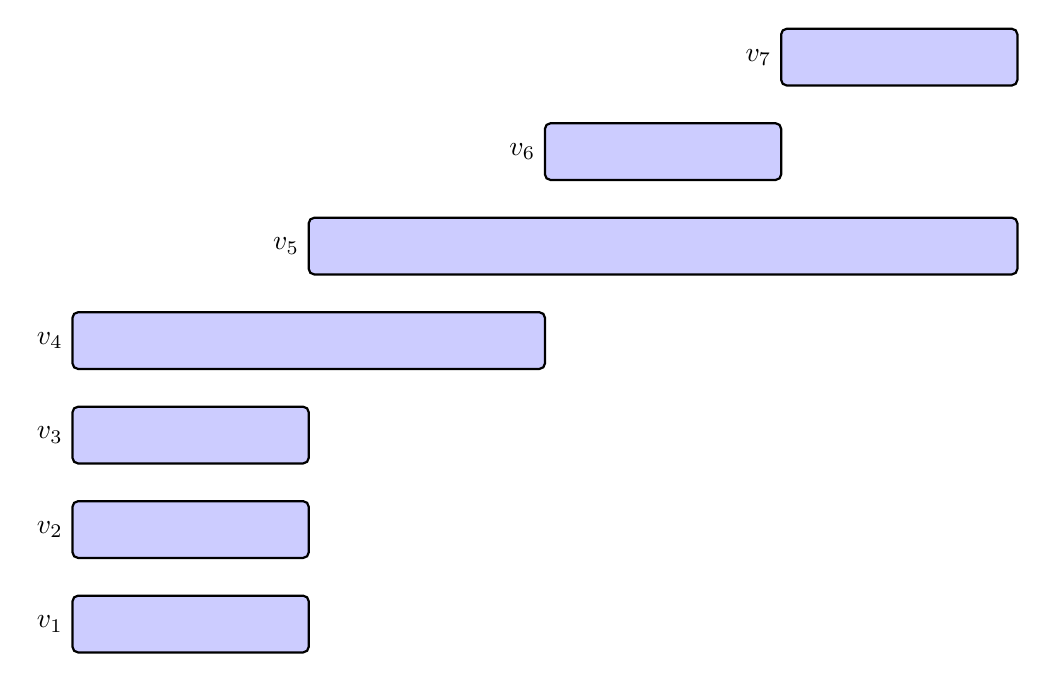
\begin{tikzpicture}[xscale=3, yscale=1.2]

		% Draw each interval as a bar
		\foreach \name/\start/\end/\y in {
				v_1/0/1/1,
				v_2/0/1/2,
				v_3/0/1/3,
				v_4/0/2/4,
				v_5/1/4/5,
				v_6/2/3/6,
				v_7/3/4/7
			} {
				\draw[thick, fill=blue!20, rounded corners=2pt] (\start,\y) rectangle (\end,\y+0.6);
				\node[left] at (\start,\y+0.3) {\(\name\)};
			}

	\end{tikzpicture}


	We see that in the proposed greedy algorithm that \(v_4\) intersects with the most amount of shifts, \(4\).

	After removing all intersections, only \(v_6, v_7\) remains, since those two are disjoint, the greedy algorithm returns volunteers \(v_4, v_6, v_7\) as its best solution.

	But notice that, by taking volunteers the two \(v_1, v_5\) we sufficiently cover all shifts in the set, thus this greedy algorithm is not optimal on all instances.

\end{soln}
\fi

	\begin{soln}
		First, define a base case, the path from \(s\) to itself will have cost zero, so long as the delay is non-negative.

		If delay is less then zero, we will give it a cost of ininfity, since delays are assumed to be non-negative.

		For the other cases, consider the last node in the path and the node that precedes it, denote it by \(u\).

		If \(u\) is going to precede it, then the path from \(s\) to \(u\) should have delay at most \(\delta - d(u, v)\).

		Since we want the minimized cost path, then \(P(\delta, v) = \min_{(u, v) \in E} (P(\delta - d(u, v), u) + p(u, v))\).

		\[
			P(\delta, v) = \begin{cases}
				0                                                      & \text{if } s = v \text{ and } \delta \geq 0 \\
				\infty                                                 & \text{ if } \delta < 0                      \\
				\min_{(u, v) \in E} (P(\delta - d(u, v), u) + p(u, v)) & \text{ otherwise }
			\end{cases}
		\]

	\end{soln}

	\question[7] Give a recursive memoized algorithm to solve for $P(D,v)$ for a given maximum delay $D$ and node $v$.

	\ifsolutions\begin{soln}
	Sort the shifts in terms of ascending order by finish time, for any ties, place first the earliest start time.

	Choose the first shift in the ordered list, and add it to our solution set.

	Then delete any intersecting shifts to that shift and remove that shift itself from the ordered list.

	Continue to the next shift in the ordered list and repeat the previous steps until the list is empty.
\end{soln}

\fi

	\begin{soln}
		Assume that all relevant functions and arrays are defined.

		I.e. weight functions for delays \(d\), cost weight functions \(p\), adjacency lists, edge lists.

		\begin{algorithmic}[1]
			\Procedure{Find-Best-Path-Wrapper}{$D, v$}
			\State Define $P[(\delta, u)] = $ min cost to reach node $u$ from $s$ with delay at most $\delta$ using a dictionary
			\State \Return Find-Best-Path($D, v, P$)
			\EndProcedure
		\end{algorithmic}

		\newpage

		\begin{algorithmic}[1]
			\Procedure{Find-Best-Path}{$\delta, u, P$}
			\If {$s = u$ and $\delta \geq 0$}
			\State \Return $0$
			\EndIf
			\If {$\delta < 0$}
			\State \Return $\infty$
			\EndIf
			\If{$P[(\delta, u)] = None$}
			\State $P[(\delta, u)] = \min_{(u', u) \in E}(\text{Find-Best-Path}(\delta - d(u', u), u', P) + p(u', u))$
			\EndIf
			\State \Return $P[(\delta, u)]$
			\EndProcedure
		\end{algorithmic}

	\end{soln}




\end{questions}
